\chapter{Ewaluacja modeli}

\section{Przebieg nauki}

\ref{rys:lstm_one_deep_comparison} tabela przedstawiająca szczegóły budowy głębokiej architektury LSTM.

\begin{figure}[t]
\centering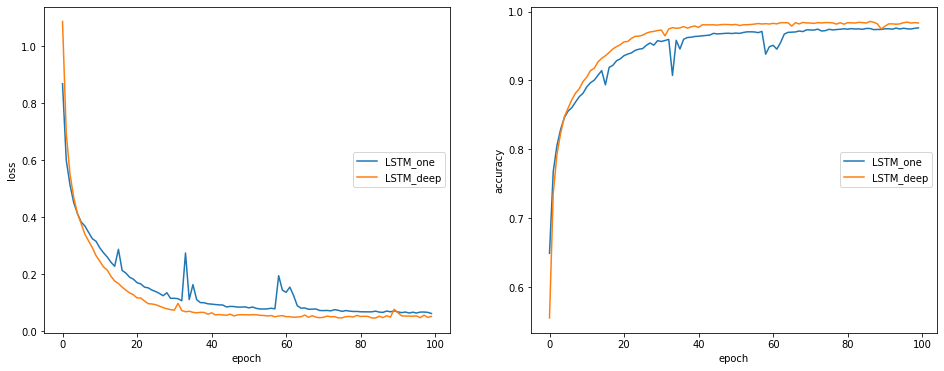
\includegraphics[width=\textwidth]{figures/reports/lstm_one_deep_comparison.png}
\fcmfcaption{Wykresy przedstawiające przebieg nauki dla modeli jednowarstwowego LSTM oraz głębokiego LSTM}\label{rys:lstm_one_deep_comparison}
\end{figure}

\section{Metryki}

TODO

\section{Wyniki}

\begin{table}[t]
\fcmtcaption{Tabela pokazująca wyniki poszczególnych modeli.}\label{tab:tabela_results}
\centering\footnotesize%
\begin{tabular}{c c c c c}
\toprule
model & dokładność & mikro precyzja & micro czułość & mikro F1 \\
\midrule
Jednowarstwowy LSTM   & 0.85 & 0.49 & 0.70 & 0.58 \\
Głęboki LSTM   & 0.87 & 0.51 & 0.71 & 0.60 \\
BERT todo   & xx & xx & xxx & xxx \\
\bottomrule
\end{tabular}
\end{table}